\documentclass[12pt,final,fleqn]{article}

% basic packages
\usepackage[margin=1in] { geometry }
\usepackage{amssymb,amsmath, bm}
\usepackage{verbatim}
\usepackage[latin1]{inputenc}
%\usepackage[OT1]{fontenc}
\usepackage{setspace}
\usepackage{natbib}
\usepackage{enumitem}
\usepackage{url}
\usepackage[font={bf}]{caption}
%\usepackage{pgfplots}
%\usepackage[font={bf}]{caption}
\usepackage{setspace}
\usepackage{latexsym}
%\usepackage{euscript}
\usepackage{graphicx}
\usepackage{marvosym}
%\usepackage[varg]{txfonts}  Older version of ``g'' in math.

% bibliography packages
\usepackage{natbib}
\bibpunct{(}{)}{;}{a}{}{,}
\bibliographystyle{apsr}
\renewcommand{\bibname}{References}

% hyperref options
\usepackage{color}
\usepackage{hyperref}
\usepackage{xcolor}
\hypersetup{
    colorlinks,
    linkcolor={blue!50!black},
    citecolor={blue!50!black},
    urlcolor={blue!80!black}
}
\newcommand*{\Appendixautorefname}{Appendix}
\renewcommand*{\sectionautorefname}{Section}
\renewcommand*{\subsectionautorefname}{Section}
\newcommand{\aref}[1]{\hyperref[#1]{Appendix~\ref{#1}}}

% packages for tables
\usepackage{longtable}
\usepackage{booktabs, threeparttable}
\usepackage{threeparttablex}
%\usepackage{tabularx}
% dcolumn package
\usepackage{dcolumn}
\newcolumntype{.}{D{.}{.}{-1}}
\newcolumntype{d}[1]{D{.}{.}{#1}}
\captionsetup{belowskip=10pt,aboveskip=-5pt}
\usepackage{multirow}
% rotating package
\usepackage[figuresright]{rotating}
\usepackage{pdflscape}
\usepackage{subcaption}

% packages for figures
\usepackage{grffile}
\usepackage{afterpage}
\usepackage{float}
\usepackage[section]{placeins}

% theorem package
\usepackage{theorem}
\theoremstyle{plain}
\theoremheaderfont{\scshape}
\newtheorem{theorem}{Theorem}
\newtheorem{algorithm}{Algorithm}
\newtheorem{assumption}{Assumption}
\newtheorem{lemma}{Lemma}
\newtheorem{proposition}{Proposition}
\newtheorem{remark}{Remark}
\newcommand{\qed}{\hfill \ensuremath{\Box}}
\newcommand\indep{\protect\mathpalette{\protect\independenT}{\perp}}
\DeclareMathOperator{\sgn}{sgn}
\DeclareMathOperator{\tr}{tr}
\DeclareMathOperator{\argmin}{arg\min}
\DeclareMathOperator{\argmax}{arg\max}
\def\independenT#1#2{\mathrel{\rlap{$#1#2$}\mkern2mu{#1#2}}}
\providecommand{\norm}[1]{\lVert#1\rVert}
\renewcommand\r{\right}
\renewcommand\l{\left}
\newcommand\E{\mathbb{E}}
\newcommand\dist{\buildrel\rm d\over\sim}
\newcommand\iid{\stackrel{\rm i.i.d.}{\sim}}
\newcommand\ind{\stackrel{\rm indep.}{\sim}}
\newcommand\cov{{\rm Cov}}
\newcommand\var{{\rm Var}}
\newcommand\SD{{\rm SD}}
\newcommand\bone{\mathbf{1}}
\newcommand\bzero{\mathbf{0}}

% dotted lines in tables
%\usepackage{arydshln}

\usepackage{pdflscape}

% spacing between sections and subsections
\usepackage[compact]{titlesec}

% times new roman
%\usepackage{times}

% appendix settings
\usepackage[toc,page,header]{appendix}
\renewcommand{\appendixpagename}{\centering Appendices}
\usepackage{chngcntr}
\usepackage{etoolbox}
\usepackage{lipsum}


% file paths and definitions
\makeatletter
\newcommand*\ExpandableInput[1]{\@@input#1 }
\makeatother

\setlength{\mathindent}{1cm}
\allowdisplaybreaks[4]
\doublespacing
%\special{pdf: pagesize width 8.5truein height 11.0truein}

\titleformat{\subsection}
  {\itshape\large}{\thesubsection}{1em}{}

\setcounter{tocdepth}{1}
\begin{document}
\author{Devin Incerti and Trevor Incerti}
\title{\textbf{Political Instability and Financial Markets}}
\date{\today}
\maketitle

\singlespacing
\begin{abstract}
We examine the relationship between political instability and daily returns of national stock indices. Financial volatility increases dramatically following (and immediately before) ``irregular'' regime changes caused by coup d'etat, assassinations, and resignations. Some of the pre-resignation volatility occurs due to actions that precede the resignation such as public protests, riots, and popular demonstrations. However, these irregular regime changes have disparate effects on the direction of stock returns. Abnormal returns following resignations are large and positive (6\%) while abnormal returns following assassinations are negative and smaller in magnitude (1\%). The impact of coups tends to be negative, but some events such as the temporary ousting of Hugo Chavez during the 2002 Venezuelan coup attempt result in positive abnormal returns of 20\% or more.
\end{abstract}
\doublespacing

\section{Introduction} \label{sec:Introduction}
For investors, multinational firms, development agencies, and aid organizations, political risk is a top consideration when making investment decisions in emerging markets. In fact, in the 2013 Multilateral Investment Guarantee Agency (MIGA) \textit{World Investment and Political Risk} report, executives of multinational enterprises (MNEs) ranked political risk as the second most important constraint for foreign direct investment (FDI) in developing countries over the next three years (after macroeconomic instability) \citep{wipr2013}. In 2011 and 2012, political risk was ranked the most important constraint for FDI in developing countries - even greater than macroeconomic instability. \footnote{The types of political risk of most concern to investors in developing countries (ranked in order of importance) were 1) adverse regulatory changes, 2) breaches of contract, 3) transfers and convertibility restrictions, 4) civil disturbances, 5) non-honoring of government guarantees, 6) expropriation nationalization, 7) terrorism and 8) war.}

A common hypothesis is that political instability discourages investment and reduces economic growth by increasing policy uncertainty. This hypothesis is supported by cross country empirical evidence that political instability - as measured by regime change frequency or political violence - is negatively correlated with investment, GDP growth, and financial development in cross country regressions \citep{alesina1996political,alesina1996income,roe2011political}. \footnote{In particular, \citep{alesina1996political} show that countries have lower growth in years in which there are major government changes such as coups. On the other hand, \citep{londregan1990poverty} finds that coups have no effect on economic growth.} However, such hypotheses are overly simplistic. Not all political instability is equivalent - resignations, assassinations, and coups are each examples of political instability, but may have disparate effects on financial returns. Further, political instability may be seen as a \textit{positive} event if the current regime is regarded as strongly anti-business or anti-global.  \citep{alesina1996political} takes the possibility of a new government adopting better economic policies seriously, but argues that the negative effects of uncertainty dominate the positive effects of coups staged by pro growth factions. 

As in \citep{alesina1996political}, we use ``irregular'' regime changes such as coups, assassinations and resignations as an indicator for political instability. The major innovation of this paper is that, in contrast to the aforementioned cross country studies, we analyze the impact of political instability using daily financial data. This enables us to use market expectations to quantify the economic impact of each individual type of regime change. The advantage of this event study approach is that it allows us to isolate the effect of irregular regime changes and mitigate the endogeneity problems that are nearly ubiquitous in cross country regressions.

We find that financial volatility increases dramatically following (and just before) coup d'etat, assassinations, and resignations. However, unlike the previously mentioned studies, we find that these irregular regime changes have disparate effects on the direction of stock returns. Abnormal returns following resignations are large and positive (6\%) while abnormal returns following assassinations are negative and smaller in magnitude (1\%). The impact of coups tends to be negative, but some events result in positive abnormal returns of 20\% or more. This finding is consistent with research that shows that ``good coups'' - coups that lead to democratization and economic liberalization - are not the norm and therefore on average coups should not be expected to lead to increased economic development and positive market returns \citep{derpanopoulos2015coups}. However, while ``good coups'' may be the minority, they do exist, and coups that attempt to overthrow anti-business autocrats may be expected to result in positive abnormal returns as investors see little risk of a replacement government ``worse'' than the status quo.

Our main finding is therefore that the type of political event and its expected impact on economic policy determines the direction of abnormal returns. Events expected to lead to more stable governance, economic liberalization, or democratization (such as willful resignations and coups that overthrow protectionist or leftist autocrats) are associated with positive returns, while those that consolidate authoritarian rule, exacerbate poor economic policies, or merely increase policy uncertainty have the opposite effect.

\bigskip

This paper is closely related to four branches of literature. The first analyzes the economic impact of political instability. This area contains a number of theoretical models in addition to the empirical work already mentioned. These models tend to focus on government policy instruments that affect private rates of return on investment. The general argument is that political instability causes governments to act myopically and adopt inefficient policies. \footnote{For instance, \citep{svensson1998investment} argues that governments are less likely to invest in the legal system and the protection of property rights when political uncertainty is high. Similarly, \citep{devereux1998political} propose a model in which political instability causes governments to leave fewer assets to their successors which forces them into increasing capital taxes. The knowledge of future taxation causes the private sector to reduce current investment which reduces future output.}

The second looks at how the variance of stock market returns reacts to political events. \citep{leblang2005government} show that right-wing governments increase the mean and volatility of stock prices in the United States and Britain. \citep{jensen2005market} find that a rise in the popularity of a Brazilian presidential candidate with uncertain future policies increased the volatility (but not the mean return) of the Brazilian stock market.

The third strand examines the impact of leaders on political and economic outcomes. \citep{jones2005leaders} identify exogenous leadership transitions using deaths of leaders from natural causes or accidents. Their results indicate that leaders influence monetary policy and economic growth. \citep{jones2009hit} find that transitions to democracy are more likely after the assassinations of autocrats.

The fourth uses event studies to assess political phenomenon. A growing body of work uses political events to estimate the effect of political connections on firm value \citep[e.g.][]{fisman2001estimating,faccio2006politically,goldman2009politically}. Studies in ``forensic economics" have used abnormal returns from political events to locate or examine transactions such as insider trading \citep{dube2011coups}, illegal arms trading \citep{dellavigna2010detecting}, and the impact of hostilities on the financial performance of diamond mining firms in Angola \citep{guidolin2007diamonds}.

\section{Data}
Political data are primarily drawn from the Center for Systemic Peace's (CSP) Polity IV Coup d'etat dataset and Coup d'etat Events handbook. The Coup d'etat dataset includes the date of 1) successful coups, 2) attempted coups, 3) plotted coups and 4) alleged coup plots. We focus on successful coups because it is difficult to classify failed coups.\footnote{\citep[p. 617]{needler1966political} has even gone so far as to say that ``the categories of coups that were aborted, suppressed, or abandoned melt into each other and into a host of other non-coup phenomena so as to defy accounting.''} As even successful coups can have disparate outcomes (e.g. a shift from authoritarian rule to democratic rule, or vica versa), we provide a list of coups and their general outcome in \autoref{tab:coup list} below. 

\singlespacing
\footnotesize
\begin{center}
\begin{longtable}[!ht]{l@{\extracolsep{\fill}}lll}
\caption{List of Coup d'Etat}
\label{tab:coup list}\\
\vspace{-5pt}\\
\hline
\multicolumn{1}{c}{Coup Date}&\multicolumn{1}{c}{Country}&\multicolumn{1}{c}{Coup Outcome}\\\hline
\endfirsthead
\multicolumn{3}{c}%
{\tablename\ \thetable\ -- \textit{Continued from previous page}} \\
\hline
\hline
\multicolumn{1}{c}{Coup Date}&\multicolumn{1}{c}{Country}&\multicolumn{1}{c}{Coup Outcome}\\\hline
\hline
\endhead
\hline 
\multicolumn{3}{r}{\textit{Continued on next page}} \\
\endfoot
\hline
\endlastfoot
06/08/1970 & Argentina & Authoritarian to authoritarian\\
03/22/1971 & Argentina & Authoritarian to authoritarian\\
03/24/1976 & Argentina & Democratic to authoritarian\\
10/06/1976 & Thailand & Democratic to authoritarian\\
10/20/1977 & Thailand & Authoritarian to authoritarian\\
12/12/1979 & South Korea & Authoritarian to authoritarian\\
02/23/1991 & Thailand & Democratic to authoritarian\\
04/05/1992 & Peru & Democratic to authoritarian\\
10/12/1999 & Pakistan & Democratic to authoritarian\\
10/04/2002 & Nepal & Democratic to authoritarian\\
09/19/2006 & Thailand & Democratic to authoritarian\\
01/11/2007 & Bangladesh & Authoritarian to authoritarian\\
04/11/2002 & Venezuela & Failed authoritarian to democratic\\
\hline
\hline
\end{longtable}
\end{center}
\doublespacing
\normalsize

The Coup d'etat Events handbook also provides a list of 1) auto-coups, 2) the ouster of leadership by foreign forces, 3) the ouster of leadership by rebel forces, 4) assassinations of the executive and 5) resignations of the executive due to poor performance and/or loss of authority. Daily financial data is available for countries in categories 4 and 5, so we supplement the coups with assassinations and resignations to form a list of ``irregular'' regime changes. The resignations are those in which the ruling executive was coerced to resign due to poor performance, public discontent and popular demonstrations.

We further supplement the CSP data with leadership data from Archigos Version 2.9, which allows us to identify additional cases in which a ``leader lost power through irregular means.'' Irregular transfers of power are those in which leaders do not leave office ``in a manner prescribed by either explicit rules or established conventions.'' Nearly all removals by irregular means result from the threat or use of force (e.g. coups, revolts and assassinations).

Financial data are from the Global Financial Data database, which includes the longest available time series of stock prices. We collect data on national equity indices and two global equity indices, the S\&P/IFC Emerging Market Investable Composite and the Morgan Stanley Capital International (MSCI) World Index. The S\&P/IFC index includes securities from emerging markets while the MSCI index includes securities from developed markets only. We collect stock index data on every country in which there was a coup or coup attempt, an assassination or failed assassination, or a forced resignation.\footnote{The list of failed assassinations are from \citep{jones2009hit}. Coup attempts are those in category 2 in the CSP Coup d'etat dataset.} The longest available time series for these stock indices are listed in \autoref{tab:stock list}.

\singlespacing
\footnotesize
\begin{center}
\begin{longtable}[!ht]{l@{\extracolsep{\fill}}lll}
\caption{List of stock indices}\label{tab:stock list}\\
\vspace{-5pt}\\
\hline
\hline
\multicolumn{1}{c}{Country}&\multicolumn{1}{c}{Stock Index}&\multicolumn{1}{c}{Begin Date}&\multicolumn{1}{c}{End Date}\\
\hline
\endfirsthead
\multicolumn{4}{c}%
{\tablename\ \thetable\ -- \textit{Continued from previous page}} \\
\hline
\hline
\multicolumn{1}{c}{Country}&\multicolumn{1}{c}{Stock Index}&\multicolumn{1}{c}{Begin Date}&\multicolumn{1}{c}{End Date}\\
\hline
\endhead
\hline \multicolumn{4}{r}{\textit{Continued on next page}} \\
\endfoot
\hline
\endlastfoot
Argentina & Beunos Aires SE General Index & Dec-66 & Jan-13\\
Australia & Australia ASX All Ordinaries & Jan-58 & Jan-13\\
Bangladesh & Dhaka SE Index & Jan-90 & Apr-09\\
Canada & Canada S\&P/TSX 300 Composite & Jan-76 & Jan-13\\
Chile & Santiago IGBC General Index & Jan-75 & Jan-13\\
Colombia & Colombia IGBC General Index & Jan-92 & Jan-13\\
Ecuador & Ecuador Bolsa de Valores de Guayaquil (BVG) & Jan-94 & Nov-11\\
Egypt & Cairo SE Index & Dec-92 & Jan-13\\
Emerging Market & S\&P/IFC Emerging Markets Investable Composite & Jul-95 & Jan-13\\
France & France CAC All-Tradable Index & Sep-68 & Jan-13\\
Greece & Athens SE General Index & Oct-88 & Jan-13\\
India & Bombday SE SENSEX & Apr-79 & Jan-13\\
Indonesia & Jakarta SE Composite Index & Apr-83 & Jan-13\\
Iran & Tehran SE Price Index & Jan-95 & Mar-12\\
Israel & Tel Aviv 100 Index & May-87 & Jan-13\\
Japan & Tokyo SE Price Index (TOPIX) & Jan-53 & Jan-13\\
Latin America & Dow Jones Latin America Index & Jan-92 & Jan-13\\
Lithuania & Lithuania Lit-10 Index & Jan-99 & May-05\\
Malaysia & Malaysia KLSE Composite & Jan-80 & Jan-13\\
Nepal & Nepal NEPSE Stock Index & Jul-97 & Jul-99\\
Netherlands & Netherlands All-Share Price Index & Jan-80 & Jan-13\\
Pakistan & Karachi SE 100 Index & Jan-89 & Jan-13\\
Paraguay & Asuncion SE PDV General Index & Oct-93 & Sep-08\\
Peru & Lima SE General Index & Jan-82 & Jan-13\\
Philippines & Manila SE Composite Index & Jan-86 & Jan-13\\
Portugal & Oporto PSI-20 Index & Jan-86 & Jan-13\\
Singapore & Singapore FTSE ST Index & Jul-65 & Jan-13\\
South Korea & Korea SE Stock Price Index  & Jan-62 & Jan-13\\
Southeast Asia & Dow Jones Southeast Asia Index & Jan-92 & Jan-13\\
Spain & Madrid SE General Index & Aug-71 & Jan-13\\
Sri Lanka & Colombo SE All-Share Index & Dec-84 & Jan-13\\
Sweden & Sweden OMX Affarsvarlden General Index & Jan-80 & Jan-13\\
Taiwan & Taiwan SE Capitalization Weighted Index & Jan-67 & Jan-13\\
Thailand & Thailand SET General Index & Apr-75 & Jan-13\\
Tunisia & Tunisia SE Index & Dec-97 & Jan-13\\
Turkey & Instanbul IMKB 100 Price Index & Oct-87 & Jan-13\\
Ukraine & Ukraine PFTS OTC Index & Jan-98 & Jan-13\\
United Kingdom & UK FTSE All-Share Index & Nov-62 & Jan-13\\
United States & Dow Jones Industrial Average & Feb-1885 & Jan-13\\
Uruguay & Bolsa de Valores de Montevideo Index & Jan-08 & Jan-13\\
Venezuela & Dow Jones Venezuela Stock Index & Jan-92 & Jul-07\\
Venezuela & Caracas SE General Index & Jan-94 & Jan-13\\
World & MSCI World Price Index & Jan-76 & Jan-13\\
Zambia & Lusaka SE Index & Jan-02 & Apr-06\\
Zambia & Zambia LuSE Index & Jan-02 & Apr-06\\
\hline
\hline
\end{longtable}
\end{center}
\doublespacing
\normalsize

To gain perspective on the relationship between irregular regime changes and the stock market, \autoref{fig:AV-DR} plots the absolute value of daily stock returns averaged across all events. Returns are for 250 trading days---approximately one calendar year---before and after regime changes.

The absolute value of returns on the event day (trading day 0) are significantly larger than on any other day. In addition, the magnitude of returns begins increasing just before the event day and remains high for a short period after it. This suggests that financial volatility increase during the days surrounding regime changes, although it does not provide any evidence on mean returns.

\autoref{sec: Irregular Regime Changes} tests these results more formally. It will first analyze coups, assassinations and resignations separately and determine whether they increase mean returns. It will then combine all irregular regime changes and estimate the effect of regime changes on the variance of returns.

\begin{figure}[!ht]
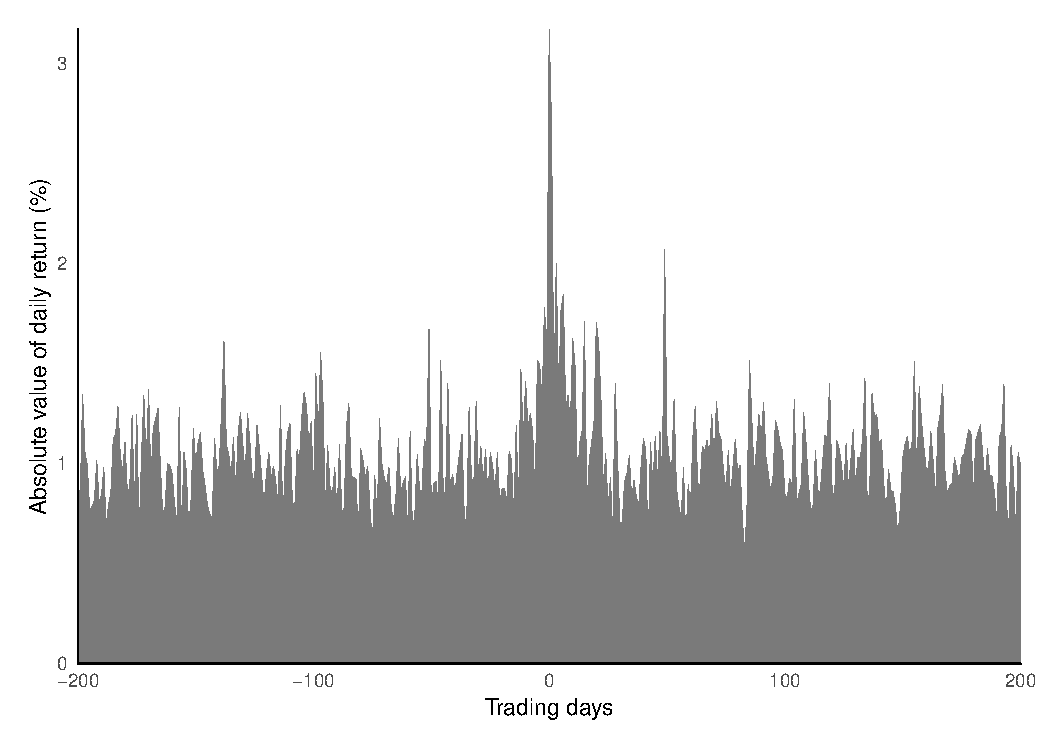
\includegraphics{../figs/daily_mean_absreturn.pdf}
\caption{Absolute value of daily returns}
\label{fig:AV-DR}
\end{figure}


\section{Irregular Regime Changes} \label{sec: Irregular Regime Changes}
\subsection{Abnormal Returns} \label{subsec: Abnormal Returns}
We begin our analysis by studying the effect of irregular regime changes on stock returns. We follow the standard event study methodology as presented by, among others, \citep{mackinlay1997event} and \citep{campbell1997econometrics}. Normal performance is measured with a constant mean return model\footnote{A constant mean return model is used instead of a market model in order to maximize the number of observations (plausible market indices such as the MSCI World Index and the S\&P/IFC Emerging Markets Investable Composite Index only begin in 1976 and 1995 respectively). That said, results are insensitive to the use of a market model.},
\begin{align} \label{eqn:market-model}
R_{it}=\mu_{i}+\epsilon_{it},
\end{align}
where $R_{it}$ is the logged return of national stock index $i$ on trading day $t$ and $\epsilon_{it}$ is the error term. We calculate abnormal returns (ARs), in an ``event window'' surrounding the date of each coup, $AR_{i\tau}=R_{i\tau}-\widehat{\mu}_i$, where $\tau$ is a date in the event window, and $\widehat{\mu}_i$ is estimated in an ``estimation window'' preceding the event window with \autoref{eqn:market-model}. We use a 41 day event window (i.e. 20 pre-event trading days, the event day, and 20 post-event trading days). The estimation window is the 250 trading days prior to the start of the event window. The abnormal returns are then used to generate cumulative abnormal returns (CARs) between event day $\tau_1$ and event day $\tau_2$: $CAR(\tau_1,\tau_2)=\sum_{\tau=\tau_1}^{\tau_2}AR_{i\tau}$.

We define the event date as the first trading day in which the market could have reacted to news of the event. For example, during the October 12, 1999 coup d'etat in Pakistan led by General Pervez Musharraf, the army announced that Prime Minister Nawaz Sharif had been dismissed after market hours at 10:15 pm. We code October 14th, the day in which the market re-opened, as the event day. When events occurred on weekends, we change the event date to the following Monday.

$(0,\tau-1)$ is used to denote the $\tau$-day period beginning with the event day and $(-1,\tau)$ to denote the negative $\tau$-day period beginning with the day prior to the event day. In other words, for cumulative abnormal returns prior to the event date, we aggregate backwards starting at the day of the event. For example, $CAR(-1,-2$) is the sum of the abnormal returns on event date $-1$ and event day $-2$.

We report abnormal returns separately for coups, assassinations and resignations because they may have distinct effects on stock returns. \autoref{tab:AR-coups} shows abnormal returns for national stock indices both preceding and following coup d'etat.
Standard errors and p-values are calculated using asymptotic t-statistics as in \citep{mackinlay1997event}. \footnote{It is appropriate to use the standard normal distribution to calculate test statistics because the length of the estimation window is sufficiently long (250 trading days).}

\begin{table}[!ht]
\caption{Abnormal returns following coups} \label{tab:AR-coups}
\vspace{-5pt}
\footnotesize
\begin{center}
\begin{threeparttable}
\begin{tabular*}{\textwidth}{l@{\extracolsep{\fill}}ld{4}d{4}d{4}d{4}d{4}d{2}}
  \hline
  \hline
\multicolumn{2}{c}{} & \multicolumn{3}{c}{Post-Event CAR} & \multicolumn{2}{c}{Pre-Event CAR} & \multicolumn{1}{c}{\multirow{2}{*}{Days to}}\\
\cmidrule(r){3-5} \cmidrule(r){6-7}
\multicolumn{1}{c}{Country} & \multicolumn{1}{c}{Event Date} & \multicolumn{1}{c}{(0,0)} & \multicolumn{1}{c}{(0,6)} & \multicolumn{1}{c}{(0,19)} & \multicolumn{1}{c}{(-1,-7)} & \multicolumn{1}{c}{(-1,-20)} & \multicolumn{1}{c}{rebound}\\
  \hline
\ExpandableInput{../tables/artable-coups-car.txt}
  \hline
\ExpandableInput{../tables/artable-coups-car-mean.txt}
   \hline
   \hline
\end{tabular*}
\scriptsize
Notes: Standard errors are in parentheses. ``Days to rebound'' is the number of trading days following a negative stock return for the national stock index to return to pre-event level (it is calculated if the price decreases on the event day, not if the event day abnormal return is negative). Returns are inflation adjusted. 
\end{threeparttable}
\end{center}
\end{table}

The average coup has a $-2.5\%$ event day AR. Event day ARs for the 1970 coup in Argentina, the 1979 coup in South Korea, the 1991 coup in Thailand, the 1992 coup in Peru, and the 1999 coup in Pakistan are all negative and statistically different than zero. Moreover, all of these cases except Thailand have negative post-event CARs and pre-event CARs that are statistically indistinguishable from zero. In all of these cases, the coup in question either overthrew a democratically elected government or changed governance from one military ruler to another. The initial negative reaction followed by additional post-event negativity is consistent with the expected market reaction from a successful authoritarian coup followed by post-event consolidation of power. 

Event day ARs are negative for all coups except the 1971 coup in Argentina and the 2002 failed coup d'etat attempt against Hugo Chavez. These results provide evidence that that coups can in fact result in positive abnormal returns. While the 1971 Argentinian coup did result in another military leader, it did so while calling for free and democratic elections and replaced a government that had adopted extreme protectionist economic policies. The ultimately failed coup against Hugo Chavez replaced a left-wing populist government with a new pro-business president.

The failed coup attempt against Hugo Chavez is a perfect natural experiment because investors reacted to an expected regime change twice: first, when Chavez was ousted, and second, when he was reinstated. On the evening of April 11, 2002, coup plotters removed Chavez from office and later detained him. Pedro Carmona, a Venezuelan economist and business leader, was named the transitional President of Venezuela. Two days later, on April 13, 2002, a popular uprising led to Chavez's reinstatement as president. This provides an estimate of the market's valuation of a transition from the Chavez regime to the Carmona regime and its valuation of a transition from the Carmona regime back to the Chavez regime. By extension, it provides an estimate of the impact of a shift from a left-wing populist government to a pro business regime in an emerging market.

\autoref{fig:AR-Ven} provides graphical evidence on the effect of the coup attempt. The top panel shows CARs for the 10 days prior to and following the event, along with 95\% confidence intervals. The daily ARs and corresponding confidence intervals are displayed in the bottom panel. The abnormal return on April 12, the first trading day in which investors could react to the coup, was 19.5\%. The market reacted similarly, albeit in the opposite direction, to Chavez's reinstatement as president: the abnormal return on the next trading day, April 15, 2002, was -14\%.

\begin{figure}[!ht]
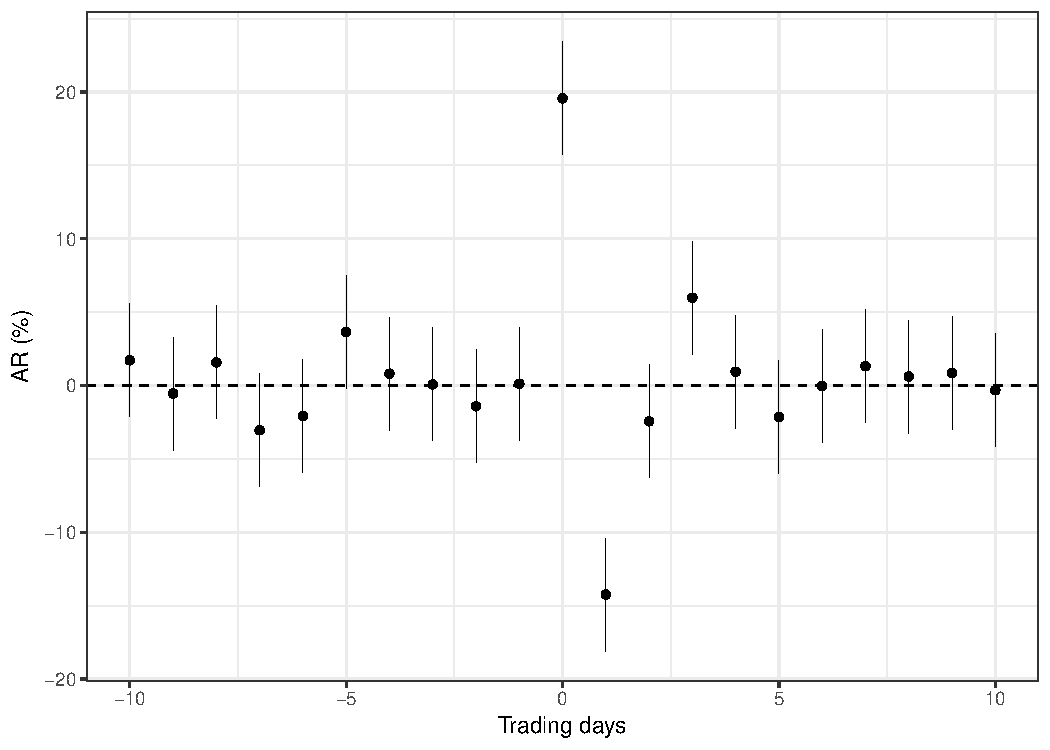
\includegraphics{../figs/venezuela_coup_attempt_2002.pdf}
\caption{Abnormal returns surrounding the 2002 Venezuelan coup d'etat attempt}
\label{fig:AR-Ven}
\end{figure}

The results in the figure are particularly striking given the discrepancy between the ARs on event days 0 and 1 and all other days. The only other day in which the ARs are statistically different from zero is on the third trading day after the coup attempt.

The almost 0\% 10-day CAR preceding the coup makes this an ideal case as it implies that investors were unaware of the coup plot. The unexpected nature of the event means that the abnormal returns capture the true value of the regime change from Chavez to Carmona more accurately than they otherwise would.

The results in \autoref{tab:AR-ass} are produced from analyses identical to those table \autoref{tab:AR-coups} but for successful assassinations rather than coups. Like the majority of coups, there is evidence that assassinations decrease stock prices. The mean event day abnormal return is negative and statistically different than zero. However, the result is driven almost entirely by three events: the shooting of U.S. President William McKinley on September 6, 1901; the assassination of U.S. President John F. Kennedy on November 22, 1963; and the assassination of Israeli Prime Minister Yitzhak Rabin on the evening of November 4, 1995.

These results are consistent with our hypothesis that the nature of the political event and its expect impact on policy matters. While the mean effect of assassinations is negative, it is smaller in magnitude than for coups. Unlike a coup, an assassination is typically a random event that will not necessarily cause immediate change in economic policy. As such, we would expect CARs to be negative due to increased instability and uncertainty, but smaller in magnitude to a coup or resignation due to greater expectations of policy inertia.

\begin{table}[!ht]
\caption{Abnormal returns following assassinations} \label{tab:AR-ass}
\vspace{-5pt}
\footnotesize
\begin{center}
\begin{threeparttable}
\begin{tabular*}{\textwidth}{l@{\extracolsep{\fill}}ld{4}d{4}d{4}d{4}d{4}d{2}}
  \hline
  \hline
\multicolumn{2}{c}{} & \multicolumn{3}{c}{Post-Event CAR} & \multicolumn{2}{c}{Pre-Event CAR} & \multicolumn{1}{c}{\multirow{2}{*}{Days to}}\\
\cmidrule(r){3-5} \cmidrule(r){6-7}
\multicolumn{1}{c}{Country} & \multicolumn{1}{c}{Event Date} & \multicolumn{1}{c}{(0,0)} & \multicolumn{1}{c}{(0,6)} & \multicolumn{1}{c}{(0,19)} & \multicolumn{1}{c}{(-1,-7)} & \multicolumn{1}{c}{(-1,-20)} & \multicolumn{1}{c}{rebound}\\
  \hline
\ExpandableInput{../tables/artable-ass-car.txt}
  \hline
\ExpandableInput{../tables/artable-ass-car-mean.txt}
   \hline
   \hline
\end{tabular*}
\scriptsize
Notes: Standard errors are in parentheses. ``Days to rebound'' is the number of trading days following a negative stock return for the national stock index to return to pre-event level (it is calculated if the price decreases on the event day, not if the event day abnormal return is negative). Returns are inflation adjusted. 
\end{threeparttable}
\end{center}
\end{table}

There is no evidence of post or pre-event CARs in almost any of the assassinations. This is consistent with expectations as assassinations are typically not predictable. As with coups, the number of days that it took the stock market to rebound to pre-event levels is fairly low.\footnote{One exception is the assassination of William Mckinley in which the stock market didn't fully recover for 963 days, or almost 4 calendar years. However, this was likely caused by the Panic of 1901, which began when the stock market crashed on May 17th, 1901, and not by McKinley's death (although the assassination may have exacerbated the panic). In any case, the length of this time period is so long that we omitted it when calculating the mean days to rebound in the figure.}

In contrast to coups and assassinations, abnormal returns following resignations are large and positive (see \autoref{tab:AR-resignations}). The mean event day abnormal return is over 6\% and event day abnormal returns are only negative and statistically significant at even the ten percent level in one out of the fifteen resignations (Tunisia on June 31, 2011). However, these positive returns are short lived: the 7 day cumulative abnormal return is nearly identical to the event day abnormal return and the 20 day cumulative abnormal return is not statistically different from zero.

\begin{table}[!ht]
\caption{Abnormal returns following resignations} \label{tab:AR-resignations}
\vspace{-5pt}
\footnotesize
\begin{center}
\begin{threeparttable}
\begin{tabular*}{\textwidth}{l@{\extracolsep{\fill}}ld{4}d{4}d{4}d{4}d{4}d{2}}
  \hline
  \hline
\multicolumn{2}{c}{} & \multicolumn{3}{c}{Post-Event CAR} & \multicolumn{2}{c}{Pre-Event CAR} & \multicolumn{1}{c}{\multirow{2}{*}{Days to}}\\
\cmidrule(r){3-5} \cmidrule(r){6-7}
\multicolumn{1}{c}{Country} & \multicolumn{1}{c}{Event Date} & \multicolumn{1}{c}{(0,0)} & \multicolumn{1}{c}{(0,6)} & \multicolumn{1}{c}{(0,19)} & \multicolumn{1}{c}{(-1,-7)} & \multicolumn{1}{c}{(-1,-20)} & \multicolumn{1}{c}{rebound}\\
  \hline
\ExpandableInput{../tables/artable-res-car.txt}
  \hline
\ExpandableInput{../tables/artable-res-car-mean.txt}
   \hline
   \hline
\end{tabular*}
\scriptsize
Notes: Standard errors are in parentheses. ``Days to rebound'' is the number of trading days following a negative stock return for the national stock index to return to pre-event level (it is calculated if the price decreases on the event day, not if the event day abnormal return is negative). Returns are inflation adjusted. 
\end{threeparttable}
\end{center}
\end{table}

These results are also consistent with the idea that the expected impact of a political event on economic policy is highly important to the directionality of returns. The positive event day abnormal return following resignations is not surprising since resignations occurred because of ``poor performance and/or loss of authority.'' Leaders were often ousted following corruption charges, financial crises, and/or political violence. For example, consider Suharto's resignation from office as the President of Indonesia on May 1998, just after the 1997 Asian Financial Crisis.

Prior to the crisis, the Indonesian economy suffered from a number of ailments including crony capitalism, poor corporate governance, growing short-term debt and a corrupt banking system \citep{radelet2000onset}. In addition, Suharto's ill health created considerable policy uncertainty, which only added to the financial panic in Indonesia. Indonesia was also hesitant to adopt structural reforms which further weakened its economic image. As a result, the crisis gave additional ammunition to opposition leaders, and public opposition culminated in riots in mid-May 1998. Suharto eventually lost his military support and was forced to resign.

\subsection{Volatility} \label{subsec: Volatility}
Although irregular regime changes have disparate effects on the direction of stock returns depending on expected policy outcomes, the results from \autoref{subsec: Abnormal Returns} suggest that all of these political events increase financial volatility. However, since stock volatility is not directly observable, one must decide how to best estimate volatility. Our estimates are obtained from a generalized autoregressive conditional heteroskedasticity (GARCH) model estimated using 1000 pre-event days, the event day and 1000 post-event days. As in \citep{jensen2005market} and \citep{leblang2005government}, we use the GARCH (1,1) specification. In particular, for national stock index $i$,
\begin{align*}
R_{it}=\mu_i + \epsilon_{it},\hspace{1cm} \epsilon_{it}\sim \mathcal{N}\left(0,\sigma_{it}^2\right),
\end{align*}
where $\mu_i$ is a constant and,
\begin{align*}
\sigma_{it}^2&=\gamma_{i}+\alpha_{i}\epsilon_{i,t-1}^2+\beta_{i}\sigma_{i,t-1}^2.
\end{align*}
The key parameter of interest is the conditional variance, $\sigma_{it}^2$. The one-period-ahead volatility forecasts, $\sigma_{it}$, are larger when $\epsilon_{i,t-1}^2$ and $\sigma_{i,t-1}^2$ are larger. In other words, the model predicts that large shocks will be followed by other large shocks.

\autoref{fig:volatility} shows the mean volatility ($\overline{\sigma_t}$) estimates from the GARCH (1,1) model across all irregular regime changes for 30 trading days prior to and 30 days after each event. Volatility appears to increase slowly just before the regime change, which suggests that investors sometimes have information about the events before they occur. Nonetheless, there is still an enormous volatility jump on the day of the regime change. Volatility then decreases to normal levels within a month of the event.

\begin{figure}[htb]
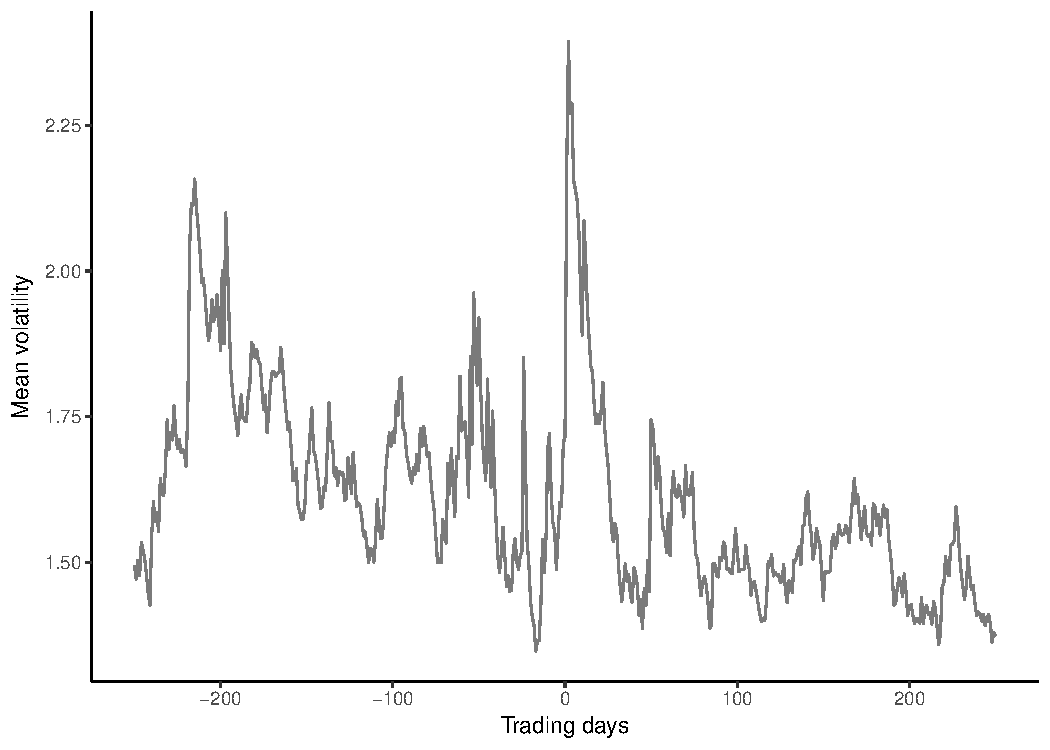
\includegraphics{../figs/mean-volatility.pdf}
\caption{Mean of volatility estimates from GARCH(1,1) models}
\label{fig:volatility}
\end{figure}

The smaller figure within \autoref{fig:volatility} expands the volatility estimates to the 250 trading days before and after each regime change. As expected, the volatility estimates stay between a narrow range at nearly all dates except those surrounding the regime change.

\subsection{Robustness} \label{subsec: Robustness}
There are three potential concerns with the results in \autoref{subsec: Abnormal Returns}. First, the abnormal returns could have been driven by factors unrelated to the regime changes. Second, the reported means are based on small sample sizes so confidence intervals based on normally distributed abnormal returns may be inappropriate. Third, the true effects of irregular regime changes on firm value may be underestimated if investors had apriori information.

To explore the first concern, we create a synthetic control portfolio for each event based on the techniques introduced in \citep{abadie2003economic} and \citep{abadie2010synthetic}. Each country is given a weight which represents its influence in the synthetic control portfolio. The weight is chosen so that the daily returns and the variance of the daily returns of the control portfolio and the event country are most similar in the estimation window. The set of possible countries in the control portfolio consists of all countries listed in \autoref{tab:stock list}.\footnote{See the appendix for a more formal explanation.}

The second concern is addressed using non-parametric statistical techniques, which are free from distributional assumptions. we employ the sign and the rank tests which are based on the sign and the rank of the event day ARs respectively.\footnote{See section 8 in \citep{mackinlay1997event} for more details.} Both tests are less influenced by departures from normality than statistics based on traditional t-tests such as those reported earlier in this paper.

\autoref{tab:non-parametric} compares event day ARs as well as ``abnormal absolute returns'' between the event country and the synthetic control portfolio using the non-parametric methods discussed above. The ``abnormal absolute returns'' are abnormal returns for the absolute value of stock returns. This is done to combine events since resignations tend to increase returns while assassinations and coups tend to decrease them. The idea that the absolute value of returns might increase during irregular regime changes is similar to the finding that volatility increases and consistent with \autoref{fig:AV-DR}.

\begin{table}[!ht]
\caption{Non-parametric tests of the impact of regime changes} \label{tab:non-parametric}
\vspace{-5pt}
\footnotesize
\begin{center}
\begin{threeparttable}
\begin{tabular*}{\textwidth}{l@{\extracolsep{\fill}}d{1.3}d{1.3}d{1.3}d{1.3}d{1.3}d{1.3}d{1.3}}
  \hline
  \hline
&\multicolumn{3}{c}{Regime Change Country}&\multicolumn{3}{c}{Synthetic Control Portfolio}&\multicolumn{1}{c}{\multirow{2}{*}{Wilcoxon}}\\
\cmidrule(r){2-4} \cmidrule(r){5-7}
&\multicolumn{1}{c}{Mean}&\multicolumn{1}{c}{Rank}&\multicolumn{1}{c}{Sign}
&\multicolumn{1}{c}{Mean}&\multicolumn{1}{c}{Rank}&\multicolumn{1}{c}{Sign}
&\multicolumn{1}{c}{Rank Test}\\
\multicolumn{1}{c}{Event Type}&\multicolumn{1}{c}{CAR (0,0)}&\multicolumn{1}{c}{p-value}&\multicolumn{1}{c}{p-value}
&\multicolumn{1}{c}{CAR (0,0)}&\multicolumn{1}{c}{p-value}&\multicolumn{1}{c}{p-value}
&\multicolumn{1}{c}{p-Value}\\
  \hline
\ExpandableInput{../tables/non-parametric-ar0.txt}
   \hline
   \hline
\end{tabular*}
\scriptsize
Notes: Estimates for assassinations do not include the assassination of U.S. president William McKinley in 1901 because no control portfolios are available. 
\end{threeparttable}
\end{center}
\end{table}

As shown in \autoref{tab:non-parametric}, the mean event day abnormal returns for coups, assassinations and resignations are all statistically different from zero at the 5\% level using the rank test statistic and the abnormal returns for coups and resignations are significant at at least the 10\% level using the sign test. In addition, abnormal absolute returns for all events are statistically significant at the 1\% level using both the rank and sign statistics. On the other hand, the event day abnormal returns for the control portfolio are never statistically different from zero at even the 10\% level. Finally, the difference in means between the regime change country and the control portfolio are statistically different from zero for coups, resignations and all events combined when using two-sided p-values from the Wilcoxon rank test.\footnote{The Wilcoxon rank test is a non-parametric statistical technique that can be used to compare differences between matched samples.} In sum, these results suggests that the results from section~\autoref{subsec: Abnormal Returns} are not an artifact of deviations from normality or confounding world events.

The third concern, which is that the political events in this paper are not unexpected, is addressed in a number of ways. First, one can note that neither the 7-day or the 20-day mean CAR from tables \autoref{tab:AR-coups}, \autoref{tab:AR-ass} or \autoref{tab:AR-resignations} are statistically different than zero at even the 10\% level. Although some of the irregular regime changes have statistically significant pre-event CAR's, most of them do not, and the ones that do not always move in the same direction. For example, there was a negative 11.8\% 7-day CAR preceding the resignation of President Estrada of the Philippines in January of 2001 and a positive 14.7\% 7-day CAR preceding the resignation of President Fernando de la Rua of Argentina in December of 2001, even though both resignations were associated with large positive event day abnormal returns.

\begin{figure}[!ht]
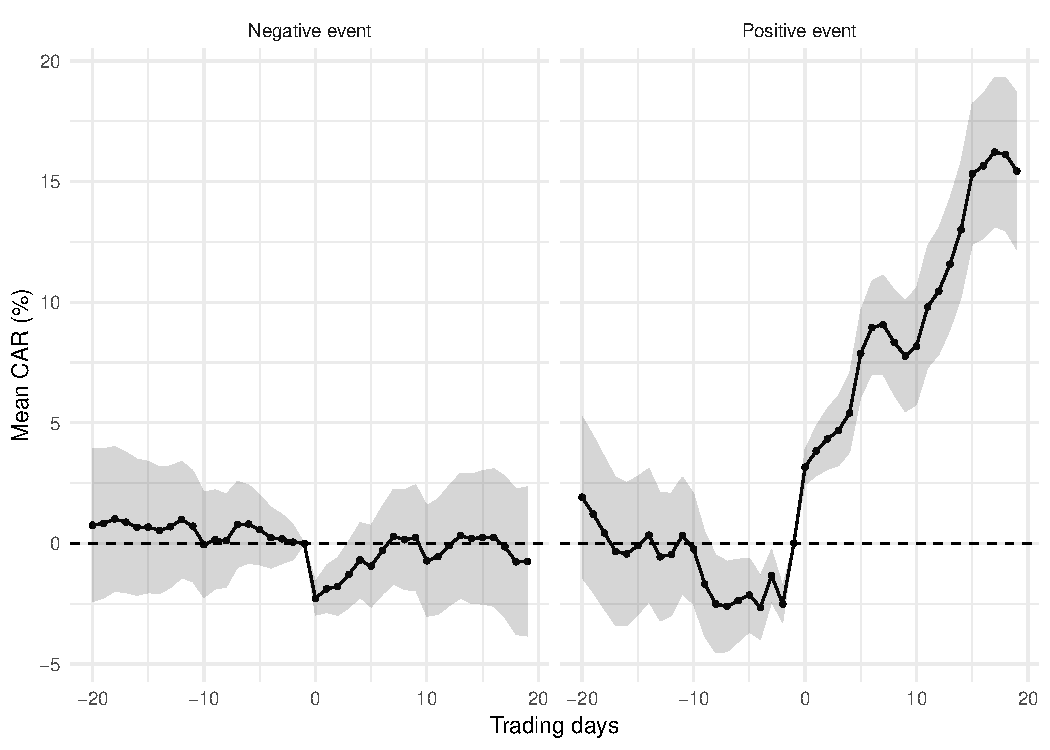
\includegraphics{../figs/mean-car-pos-neg.pdf}
\caption{Mean cumulative abnormal returns surrounding regime changes}
\label{fig:CAR-mean}
\end{figure}

Second, since the direction of the pre-trends is unclear, we examine whether there are different pre-trends for events with positive stock reactions than for events with negative stock reactions. As shown in \autoref{fig:CAR-mean}, neither the ``positive'' nor ``negative'' events have pre-event CAR's that are statistically different from 0.

It is also worth noting that the post-event CAR(1,k) for $k\in(2,19)$ is not statistically significant for either the ``positive'' or the ``negative'' events. Almost all of the stock-market reaction occurs on the first day that the market could react to the event which suggests that markets respond quickly to political events. This, in turn, implies that markets are reacting to news efficiently and that an event-driven trading strategy would not be profitable.

Fianlly, to check whether our results are sensitive to model specificaiton, we estimated market models in addition to the baseline constant returns model. We used the MSCI World Index as a proxy for ther market return. [To do: add table for this]  

\section{Public Protests} \label{sec: Public Protests}
The resignations studied in this paper are those in which leaders left office because of poor performance, public discontent and popular protests. While the previous section showed that the resignations themselves had large effects on stock returns and volatility, it is not unreasonable to expect the political actions preceding the resignations to have similarly large effects on financial markets. Indeed, corporate investors in the 2011 MIGA \textit{World Investment and Political Risk} ranked civil disturbances as the fourth most concerning type of political risk.

The most recent example of a popular uprising preceding a resignation is the 2011 Egyptian Revolution that resulted in the overthrow of President Hosni Mubarak's regime.\footnote{Abnormal returns for this event are not shown in \autoref{tab:AR-resignations} because the stock market was closed on the day of Mubarak's resignation.} Clashes between security forces and protestors led to the deaths of hundreds of citizens and injuries to thousands more. The uprising began on January 25, 2011 when millions of protestors demanded the overthrow of the Egyptian leadership. Examples of public discontent included demonstrations, marches, riots and non-violent civil disobedience, and labor strikes.

While the Egyptian Revolution may have positive pro-democracy effects on the Egpytian political system, its short-term impact on the economy was disastrous. As shown in \autoref{fig:CAR-Egypt}, abnormal returns on the Egyptian Stock Exchange Index (EGX 30) were around -7\% on January 26th and -10\% the day after. To prevent further decline during the uprising, the Egyptian Stock Exchanged closed at the end of trading on January 27th. President Mubarak resigned on February 11, but the market remained closed until March 23, when CARs declined by another 9\%, before rebounding slightly thereafter.

\begin{figure}[!ht]
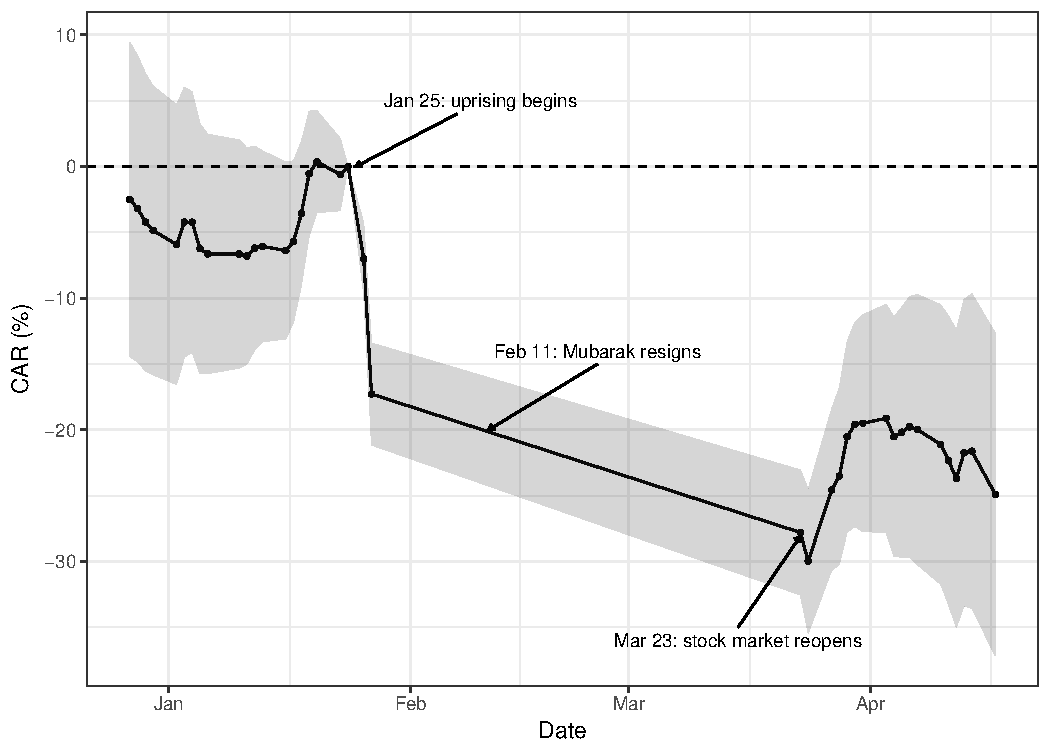
\includegraphics{../figs/egypt-revolution-2011.pdf}
\caption{Cumulative abnormal returns during the Egyptian revolution}
\label{fig:CAR-Egypt}
\end{figure}

An important question is whether other popular uprisings have had similar adverse economic consequences. To examine this, we explore all resignations that were driven by significant public protests.\footnote{The set of resignations includes all those listed in either the Coup d'etat Events Handbook or the Archigos Version 2.9 data set with available financial data. In practice, this is the 2011 Egyptian Revolution and the list or resignations in \autoref{tab:AR-resignations}.} Public protests include popular demonstrations, riots, non-violent civil resistance and other forms of public discontent. These events are listed in \autoref{tab:protest-list} in the appendix.

The start and end dates in \autoref{tab:protest-list} are the dates that protests began and leader's resigned respectively. Resignations caused by popular uprisings were identified by examining the descriptions in the Coup d'?tat Events Handbook and Archigos Version 2.9. Additional Lexis Nexis searches were used to verify these descriptions. Start dates were determined through similar means.

In \autoref{tab:protest-stocks}, we examine whether public protests influence stock prices. The variable, \textit{Protest} is equal to 1 during the dates in which citizens participate in political activities demanding the resignation of the executive are and 0 otherwise. Non-protest dates are the 250 days prior to the start dates and after the end dates listed in \autoref{tab:protest-list}.\footnote{The volatility estimates used as the dependent variable in column (4) are estimated on the 250 days prior to the start date, the protest dates, and the 250 days following the end date.}

Column (1) suggests that public protests have no effect on stock returns. However, this occurs because some political movements increase stock prices while others decrease them. As shown in column (2), the absolute value of stock returns are over 2\% higher during public protests. These estimates would be biased if protest dates are correlated with higher world or regional stock market indices. To address this potential confounder, column (3) controls for returns on the S\&P/IFC Emerging Markets Investable Composite Stock Index. The coefficient on \textit{Protest} barely changes and the absolute value of returns are still about 2\% higher during public protests. Finally, column (4) shows that stock volatility is more than 1 percentage point higher during political movements.

\begin{table}[!ht]
\caption{Effect of public protests on stock prices} \label{tab:protest-stocks}
\vspace{-5pt}
\footnotesize
\begin{center}
\begin{threeparttable}
\begin{tabular*}{\textwidth}{l@{\extracolsep{\fill}}d{1.3}d{1.3}d{1.3}d{1.3}}
  \hline
  \hline
\multicolumn{1}{c}{}&\multicolumn{1}{c}{Returns} & \multicolumn{2}{c}{Absolute Value of Returns}&\multicolumn{1}{c}{Volatility}\\
\cmidrule(r){2-2} \cmidrule(r){3-4} \cmidrule(r){5-5}
 & \multicolumn{1}{c}{(1)}&\multicolumn{1}{c}{(2)}&\multicolumn{1}{c}{(3)}&\multicolumn{1}{c}{(4)}\\
  \hline
\ExpandableInput{../tables/protest-regtable.txt}
   \hline
   \hline
\end{tabular*}
\scriptsize
Notes: Standard errors clustered by event are in parentheses. Statistical significance at the 10\%, 5\%, and 1\% level is denoted by *, ** and *** respectively.
\end{threeparttable}
\end{center}
\end{table}

\section{Conclusion}
This paper has examined the economic effects of irregular regime changes. It uses an event study approach to show that investors expect irregular regime changes to have large effects on equity returns. This methodology is less susceptible to endogeneity biases than studies that use cross country data.

The results are consistent with the idea that government competence is a random walk and that government changes have large impacts on investor confidence. Financial volatility surrounding regime changes, which is often characterized by large positive \textit{and} negative stock returns, suggests that irregular regime changes increase policy uncertainty. The variation in the direction of abnormal returns is consistent with the idea that not all governments are created equally. Abnormal returns are likely positive following resignations because those leaders were the most likely to be ``bad'' leaders.

Although this study is based on only 35 events, the size of the effects suggests that it should not be dismissed. Irregular regime changes are important economic events than can drastically alter the economic landscape. For instance, the 21.26\% increase in the Venezuelan Stock Index following the temporary ousting of Hugo Chavez in 2002 is its 4th largest increase since 1994. In comparison, the Hong Kong Stock Index (Hang Seng Index) decreased by 21.7\% following the 1989 massacre of Chinese protestors in Tiananmen square and the Dow Jones Industrial Average in the United States fell by 22.61\% on Black Monday (1997), the largest one-day drop in its history.

\appendix
\setcounter{table}{0}
\renewcommand\thetable{\Alph{section}.\arabic{table}}
\section{Appendix} \label{Appendix}
\begin{table}[!ht]
\caption{List of public protests preceding resignations} \label{tab:protest-list}
\vspace{-5pt}
\footnotesize
\begin{center}
\begin{threeparttable}
\begin{tabular*}{\textwidth}{l@{\extracolsep{\fill}}llll}
  \hline
    \hline
\multicolumn{1}{c}{Country}&\multicolumn{1}{c}{Name}&\multicolumn{1}{c}{Start Date}&\multicolumn{1}{c}{End Date}\\
  \hline
Philippines & EDSA 1/Yellow Revolution & 2/22/1986 & 2/25/1986\\
Bangladesh & Bangladeshi Spring of 1990 & 11/27/1990 & 12/7/1990\\
Thailand & Black May & 5/17/1992 & 5/20/1992\\
Indonesia & Indonesian Riots & 5/12/1998 & 5/21/1998\\
Philippines & EDSA II & 1/17/2001 & 1/20/2001\\
Argentina & Argentina Riots & 12/16/2001 & 12/20/2001\\
Ukraine & Orange Revolution & 11/22/2004 & 1/23/2005\\
Ecuador & Ecuadorian Protests & 4/13/2005 & 4/20/2005\\
Nepal & Nepalese People's Revolution & 4/6/2006 & 4/24/2006\\
Tunisia & Tunisian Revolution & 12/18/2010 & 1/14/2011\\
Egypt & Egyptian Revolution & 1/25/2011 & 2/11/2001\\
   \hline
   \hline
\end{tabular*}
\scriptsize
\end{threeparttable}
\end{center}
\end{table}

\subsection{Synthetic Control Portfolio}
Let $\boldsymbol{R}_{k}$ be the vector of returns for the event country in the estimation window, $\boldsymbol{R}_{-k}$ be the vector of returns for all other countries in the estimation window, $\boldsymbol{X}_1=(\boldsymbol{R}_{k},\var(\boldsymbol{R}_{k}))$, $\boldsymbol{X}_0=(\boldsymbol{R}_{-k},\var(\boldsymbol{R}_{-k}))$, and $\boldsymbol{W}_{-k}$ be a $((N-1) \times 1)$ vector of weights where $N$ is the number of countries listed in \autoref{tab:stock list}. Then $\boldsymbol{W}^*$ is chosen to minimize $(\boldsymbol{X}_1-\boldsymbol{X}_0\boldsymbol{W})'\boldsymbol{V}(\boldsymbol{X}_1-\boldsymbol{X}_0\boldsymbol{W})$ subject to $w_i\geq0$ $(i = 1,2,\ldots,N-1)$ and $\sum_i^{N-1} w_i = 1$, and the vector $\boldsymbol{V}$ is chosen so that stock returns for the control portfolio during the estimation window are are close as possible to the event country.\footnote{See \citep{abadie2003economic} for further details.}

\pdfbookmark[1]{References}{References}
\bibliography{bibliography}

\end{document} 